\chapter{Results}
\label{chapter6}

The task of segmenting aneurysms in TOF-MRA images is evaluated with the use of three metrics: Dice Similarity Coefficient (DSC), Modified Hausdorff Distance (MHD) (95\textsuperscript{th} percentile), and Volumetric Similarity (VS). The overlap of the prediction and ground truth segmentation map is evaluated using DSC. Compared to DSC, MHD is a distance metric and is sensitive to the overall shape of the segmentation. As the name implies, VS is a measure that considers volumes of the segmentations to indicate similarity. These are reported for the networks described in Chapter \ref{chapter4} -- DeepMedic, and nnU-Net -- and for Triplanar-Net. The metrics are evaluated using two datasets -- train, and test. The train dataset comprises the publicly available data from the ADAM challenge, and the test dataset the non-publicly available data from the same \cite{Timmins2020}. During training of all networks, the train dataset was randomly split into training and validation sets while ensuring that the distribution of positive to negative scans is maintained. To note, in the results shown in the following sections when referring to the ``train dataset'', this actually means the validation split that was manually taken from the publicly available train dataset as part of the ADAM challenge \cite{Timmins2020}. Therefore the reported results are on cases which each network was not trained on. The results were obtained on the test dataset by submitting docker containers of the method to \citeauthor{Timmins2020}, as the test dataset is not publicly available. The evaluation is done by the authors of the challenge, and the metric results are reported. It is not possible to run the further analyses on the results of the test dataset, and thus these are only evaluated for the train dataset.

Each segmented voxel or connected component of voxels is considered a positive detection. A positive detection corresponding to an aneurysm is considered a true-positive finding, whereas a positive detection not corresponding to an aneurysm was considered a false-positive finding.

The number of parameters of each network, and the inference time for a scan is also reported. Inference time per case is reported without taking into account time required for preprocessing of the data. It should be noted that DeepMedic runs on a Tensorboard backend, whereas the other networks use PyTorch. 

It is also interesting to further analyze the results with respect to each network: results such as the segmentation performance of true UIAs, segmentation performance based on size of UIAs, and performance on negative scans are also assessed. It is not possible to perform these assessments on the test dataset as it is not publicly available, so the reporting is done only on the train dataset. 
 
\section{Metrics}
Results are shown for the segmentation metrics evaluated on the full TOF-MRA volumes in Table \ref{table:metrics_full} for both the train set and the test set. The interobserver results are taken from the study performed by \citeauthor{Timmins2020}, which are found based on measurements made by two separate observers on a subset of the scans. Figure \ref{fig:results} shows the box plots of the segmentation metrics for the evaluated networks.


\begin{table}[htp]
	\centering
	\begin{tabular}{ l  r r r | r r r }
		\multirow{3}{4em}{} & \multicolumn{3}{ c |}{\textbf{Train}} & \multicolumn{3}{| c }{\textbf{Test}} \\

		& \multirow{2}{2em}{DSC} & MHD & \multirow{2}{2em}{VS} & \multirow{2}{2em}{DSC} & MHD & \multirow{2}{2em}{VS} \\
		& & (mm) & & & (mm) & \\
		\hline

		nnU-Net & \textbf{0.81} & \textbf{0.49} & \textbf{0.89} & \textbf{0.41} & \textbf{8.96} & 0.50 \\
		DeepMedic & 0.11 & 59.70 & 0.33 & 0.07 & 71.41 & 0.34 \\
		Triplanar-Net & 0.14 & 53.90 & 0.42 & 0.11 & 62.35 & \textbf{0.53} \\
		interobserver & N/A & N/A & NA & 0.63 & 2.42 & 0.76 \\
	\end{tabular}

	\caption[Segmentation results.]{The mean segmentation metrics of each network architecture evaluated on the publicly available train dataset and the test dataset. Results in bold show the best value for that specific metric for the evaluated network architectures.}
	\label{table:metrics_full}
	
\end{table}

\begin{table}[hp]
	\centering
	\begin{tabular}{ l  r r | r r }
		\multirow{3}{4em}{} & \multicolumn{2}{ c |}{\textbf{Train}} & \multicolumn{2}{| c }{\textbf{Test}} \\
		
		& False Positive Count & Sensitivity & False Positive Count & Sensitivity \\
		\hline
		
		nnU-Net & \textbf{0.00} & \textbf{0.96} & \textbf{0.18} & 0.61 \\
		DeepMedic & 99.41 & 0.90 & 118.86 & \textbf{0.85} \\
		Triplanar-Net & 28.17 & 0.84 & 31.80 & 0.76 \\
	\end{tabular}
	\caption[Detection results.]{The mean detection metrics of each network architecture evaluated on the publicly available train dataset and the test dataset. Results in bold show the best value for that specific metric.}
	\label{table:metrics_detect}
\end{table}

\begin{figure}[htp]
	\centering
	\begin{subfigure}{.6\linewidth}
		\includegraphics[width=\linewidth]{figures/DSC.eps}
	\end{subfigure}
	\begin{subfigure}{.6\linewidth}
		\includegraphics[width=\linewidth]{figures/MHD.eps}
	\end{subfigure}
	\caption[Plots of results of train dataset.]{Box plots pf results shown for DSC, MHD, VS and false positives for each network architecture for the train dataset and bar plot shown for sensitivity of detections among network architectures.}
	\label{fig:results}
\end{figure}
\begin{figure}
	\ContinuedFloat
	\centering
	\begin{subfigure}{.6\linewidth}
		\includegraphics[width=\linewidth]{figures/VS.eps}
	\end{subfigure}
	\begin{subfigure}{.6\linewidth}
		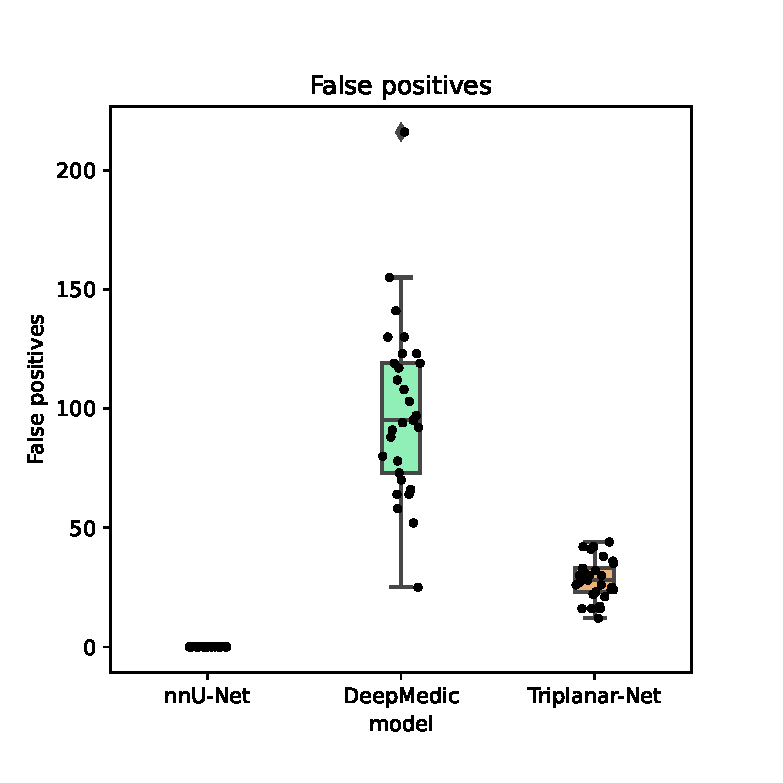
\includegraphics[width=\linewidth]{figures/FalsePositives.eps}
	\end{subfigure}
	\caption{Box plots of results shown for DSC, MHD, VS and false positives for each network architecture for the train dataset and bar plot shown for sensitivity of detections among network architectures (cont.).}
	\label{fig:results_cont}
\end{figure}
\begin{figure}
	\ContinuedFloat
	\centering
	\begin{subfigure}{.6\linewidth}
		\includegraphics[width=\linewidth]{figures/Sensitivity.eps}
	\end{subfigure}
	\caption{Box plots of results shown for DSC, MHD, VS and false positives for each network architecture for the train dataset and bar plot shown for sensitivity of detections among network architectures (cont.).}
	\label{fig:results_cont_cont}
\end{figure}

\section{Further evaluation}

\subsection{Inference}
Inference time and number of parameters of the three network architectures are shown in \ref{table:inference}; inference time is a very dependent result and to attempt to keep it as unbiased and normalized as possible, for all networks inference was done on an NVIDIA P100 GPU under equivalent conditions. The mean inference time is reported in seconds and calculated by taking an average of the time required for the forward pass of the network over all train data.

\begin{table}[h!tp]
	\centering
	\begin{tabular}{l r r }
		& parameters & mean inference time (s) \\
		\hline
		nnU-Net & 178297920 & 203 \\
		DeepMedic & \textbf{1178100} & 175 \\
		Triplanar-Net & 1478264 & \textbf{35} \\
	\end{tabular}
	\caption[Number of parameters and inference time.]{The number of parameters and mean inference time --for the forward pass -- of each network architecture across all train dataset cases.}
	\label{table:inference}
\end{table}

\subsection{Segmentation results of true UIAs}
For the three networks assessed, the segmentation performance for only true UIAs  was also evaluated, and the results are shown in Table \ref{table:metrics_pos}. This evaluation was only done on the train dataset.

\begin{table}[h]
	\centering
	\begin{tabular}{ l  r r r }
%		\multirow{3}{4em}{} & \multicolumn{3}{ c }{\textbf{Train}} \\
%		
		& \multirow{2}{2em}{DSC} & MHD & \multirow{2}{2em}{VS} \\
		& & (mm) & \\
		\hline
		%		3D U-Net & 0. & 0. & 0. & 0. & 0. & 0. \\
		nnU-Net & \textbf{0.91} & \textbf{0.47} & \textbf{0.88} \\
		DeepMedic & 0.25 & 7.99 & 0.37 \\
		Triplanar-Net & 0.23 & 10.07 & 0.27 \\
	\end{tabular}
	\caption[Segmentation results of true UIAs.]{The mean segmentation metrics of each network architecture evaluated on only true UIAs. Results in bold show the best value for that specific metric.}
	\label{table:metrics_pos}
\end{table}

\subsection{Performance on negative scans}
The average false positive count over all scans containing no true UIAs is shown in Table \ref{table:metrics_neg}, along with the false positive count for all scans. These results are only shown for the train dataset.

\begin{table}[h]
	\centering
	\begin{tabular}{ l  r r r }
		& All scans & Positive scans & Negative scans \\
		\hline
		nnU-Net & \textbf{0.00} & \textbf{0.00} & \textbf{0.00} \\
		DeepMedic & 99.41 & 97.04 & 110.80 \\
		Triplanar-Net & 28.17 & 28.00 & 29.00 \\
	\end{tabular}
	\caption[False positive count for all scans, positive scans and negative scans.]{The false positive count of each network architecture over all train cases for all scans, positive scans, and negative scans. Results in bold show the best value for that specific metric.}
	\label{table:metrics_neg}
\end{table}

\subsection{Sizes of UIAs}
In Figure \ref{fig:DSC_sizes.eps} diameter of the UIAs is split into four quartiles, and a bar plot of the DSC for the three evaluated networks is shown.

\img{DSC_sizes.eps}{0.6\linewidth}{Dice Score Coefficient of networks split into sizes of aneurysms.}{Box plot of the Dice Score Coefficients of each network architecture based on different UIA sizes, split into four quartiles.}

\subsection{Qualitative results}
Axial slices of three input TOF-MRA volumes overlayed with the segmented aneurysm are shown in Figure \ref{fig:qual_results} along with the ground truth labels.

\begin{figure}[htp]
	\centering
	\begin{subfigure}{\linewidth}
		\includegraphics[width=\linewidth]{figures/results_10049F.pdf}
	\end{subfigure}
	\begin{subfigure}{\linewidth}
		\includegraphics[width=\linewidth]{figures/results_10034.pdf}
	\end{subfigure}
	\begin{subfigure}{\linewidth}
		\includegraphics[width=\linewidth]{figures/results_10073F.pdf}
	\end{subfigure}
	\caption[Qualitative results of each network on three positive cases.]{The axial slices of three positive TOF-MRA volumes, showing the ground truth labels, the output segmentation of the nnU-Net architecture, the output segmentation of the DeepMedic architecture, and the output segmentation of the Triplanar-Net architecture in each row respectively.}
	\label{fig:qual_results}
\end{figure}